\chapter{Testowalność aplikacji Android}
\label{opis_problemu}

\section{Pojęcie architektury w~kontekście systemów \newline komputerowych}
\subsection{Architektura systemowa}
Systemy komputerowe są kombinacjami sprzętu, oprogramowania i~sieci komponentów. Termin \textit{"architektura systemu"} opisuje strukturę, interakcję i~technologię komponentów systemu komputerowego, w~tym także oprogramowania.

Systemy oprogramowania są skonstruowane tak, aby spełnić cele biznesowe organizacji. Architektura systemowa jest określana jako abstrakcyjny pomost między tymi celami. Choć droga od abstrakcyjnych celów do konkretnych systemów może być złożona, dobrą wiadomością jest to, że architektura oprogramowania może być zaprojektowana, przeanalizowana, udokumentowana i~realizowana przy użyciu znanych technik, które przyczynią się do osiągania tych celów biznesowych i~misji twórcy. 


\subsection{Architektura oprogramowania}
Istnieje wiele definicji architektury oprogramowania. Na potrzeby tej pracy autor wybrał przedstawioną w~książce Lena Bassa, Paula Clementsa i~Ricka Kazmana "Software Architecture in Practice"\cite{bib:architect:software} \textit{Architektura oprogramowania jest zbiorem struktur potrzebnych do uporządkowania systemu, które zawierają elementy oprogramowania i~sprzętu oraz opisują relacje między nimi}. 

W systemach opartych na modelu \textit{waterfall}, architekturę oprogramowania tworzona jest przed rozpoczęciem kodowania i~jest to bardzo poważny proces, który mógł wpłynąć na losy projektu. w~modelach projektowych opartych na metodykach zwinnych, do których autor nawiązuje i~przekonuje w~tej pracy, architektura oprogramowania może być zmieniana również podczas tworzenia systemu. Czasem jest to nawet niezbędne ze względu na dynamiczne zmiany w~wymaganiach użytkownika, lub pojawianie się kolejnych \textit{use cases}.

Oto wnioski wynikające z~przytoczonej wcześniej definicji:

\paragraph{Architektura jest zbiorem struktur oprogramowania}

Struktura jest zbiorem elementów spojonych ze sobą relacjami. Systemy oprogramowania składają się z~wielu struktur, ale żadna pojedyncza struktura nie jest jeszcze architekturą. Istnieją trzy kategorie struktur architektonicznych, które odgrywają ważną rolę w~zakresie projektowania, dokumentowania i~analizy architektur:
\begin{itemize}
\item
Niektóre systemy dzielą struktury na mniejsze jednostki wykonawcze, które zwykle nazywane są modułami. Modułom przypisane są konkretne zadania obliczeniowe, które stają się podstawą przypisania pracy dla zespołów programistycznych. w~przypadku dużych projektów, elementy te (moduły) mogą być podzielone na jeszcze mniejsze części w~celu przypisania do podrzędnych zespołów. Na przykład, zaprojektowanie bazy danych dla systemu zarządzania gospodarką magazynową, produkcją, księgowością i~zasobami ludzkimi (ERP\footnote{ERP - Enterprise Resource Planning (ang.) – planowanie zasobów przedsiębiorstwa}) w~dużym przedsiębiorstwie może być zbyt skomplikowane dla jednego zespołu i~realizacja tego celu musi zostać podzielona na wiele części. Moduł logistyczny może stać się jednym modułem, moduł produkcyjny drugim, itd. Również inne funkcjonalności systemu muszą czasem zostać podzielone i~przypisane do osobnych zespołów wdrożeniowych.
\item
Inne struktury systemowe mogą być dynamiczne, co oznacza, że dotyczą sposobu, w~jaki poszczególne elementy współdziałają ze sobą w~czasie wykonywania planowanych funkcji systemu. Jeżeli system ma być zbudowany jako zestaw usług, to usługi te współdziałają z~infrastrukturą i~wymagają synchronizacji. 

\item
Trzeci rodzaj struktury opisuje odwzorowanie elementów softwarowych na elementy systemowe: organizacyjne, instalacyjne, uruchomieniowe i~rozwojowe. Na przykład, moduły mogą być przypisane do zaprogramowania przez zespoły oraz przypisane do odpowiednich miejsc w~strukturach systemu, tak aby później nie było problemów chociażby z~ich testowaniem.
Te odwzorowania nazywane są \textit{alokacyjnymi}.

\end{itemize}

\paragraph{Architektura jest pojęciem abstrakcyjnym}
Ponieważ architektura zawiera struktury, a~struktury te zawierają elementy i~relacje między nimi, wynika z~tego że architektura łączy te elementy systemowe ze sobą wykorzystując relacje. Oznacza to, że architektura pomija pewne informacje, które nie są użyteczne z~punktu widzenia systemu, a~w szczególności takie, które nie są ze sobą powiązane żadną relacją. Zatem architektura jest przede wszystkim abstrakcją systemu, który wybiera pewne szczegóły i~ukrywa inne. We wszystkich nowoczesnych systemach elementy współdziałają ze sobą za pomocą interfejsów, które dzielą dany element na części publiczne i~prywatne (wewnętrzne). Architektura zajmuje się stroną publiczną tego podziału, a~prywatne interakcje między funkcjami, czy nawet funkcje pełniące tylko zadania pomocnicze, nie są elementem architektonicznym. Taki rodzaj abstrakcji jest niezbędny do opisania systemu w~możliwie najprostszy i~zrozumiały sposób.

\paragraph{Każdy system softwarowy posiada architekturę oprogramowania}
Każdy system można pokazać w~sposób opisany w~poprzednich paragrafach, czyli jako zestaw elementów i~relacji między nimi. w~najprostszym przypadku - cały system będzie pojedynczym elementem, ale architektura opisana w~ten sposób będzie bezużyteczna.

Nawet jeżeli każdy system posiada architekturę, to nie znaczy, że architektura ta jest znana. Zdarza się, że ludzie, którzy ją tworzyli, już nie pracują, a~dokumentacja zaginęła lub, co gorsze, w~ogóle nie była tworzona. Jeśli do tego kod źródłowy nie został zachowany, zostaje tylko binarny kod wykonywalny, który niekoniecznie może być pomocny przy analizie systemu.
Różnica pomiędzy architekturą systemu a~jej reprezentacją polega na tym, że architektura może istnieć niezależnie od specyfikacji systemu.  Warunkiem koniecznym do odtworzenia systemu jest jej zapisana dokumentacja.

\paragraph{Architektura obejmuje również zachowanie systemu}
Zachowanie się każdego elementu architektury może być również jej częścią, o~ile czynność ta wnosi jakieś nowe informacje i~wpływa pozytywnie na zrozumienie systemu. Reprezentowanie, jak elementy współdziałają ze sobą, jest częścią definicji architektury, opisanej w~poprzednich paragrafach. Rysunki typu \textit{box-and-line}, które często przedstawiane są jako architektura systemu, w~gruncie rzeczy nią nie są. Patrząc na nazwy pól (bazy danych, graficzny interfejs użytkownika, etc.), można sobie wyobrazić funkcjonalność i~zachowanie odpowiednich elementów, ale wypływają one w~większości z~wyobraźni obserwatora i~nie opierają się na żadnej udokumentowanej informacji. To nie znaczy, że dokładne zachowanie i~wydajność każdego elementu muszą być udokumentowane w~każdym przypadku - niektóre zachowania systemu nie leżą w~grupie zainteresowań architekta. Jednak jeżeli interakcja pomiędzy poszczególnymi elementami jest kluczowa dla działania systemu - powinna ona zostać udokumentowana.

\paragraph{Nie wszystkie rodzaje architektur są odpowiednie}
Definicja architektury nie specyfikuje niestety, która architektura jest dla danego systemu odpowiednia bądź nie - lub - mówiąc bardziej dosadnie, która jest dobra, a~która zła. Jak autor wykaże w~kolejnych rozdziałach, również w~przypadku systemu Android wybór odpowiedniej architektury jest kluczowy dla testowalności i~pielęgnowalności  oprogramowania tworzonego dla tej platformy.

\section{Architektura Android}
Architektura Android przez wielu opisywana jest jako \textit{Java on Linux}, czyli programowanie w~Javie pod Linuksem. Jednakże jest to stwierdzenie zbyt ogólne, biorąc pod uwagę złożoność całej platformy. Całość systemu zawiera bowiem w~sobie komponenty, które układają się w~pięć głównych warstw: \textit{Android applications}, \textit{Android Framework}, \textit{Dalvik virtual machine}, \textit{user-space native code} oraz \textit{Linux kernel}\cite{bib:hacker:handbook}.

\begin{figure}[!htb]
    \centering
    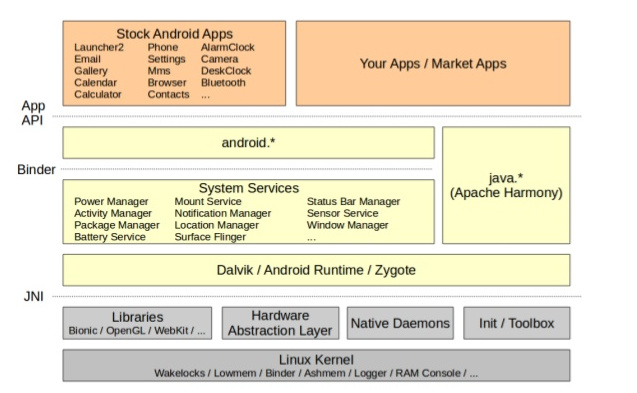
\includegraphics[width=14cm]{imgs/ch3_android_architecture_1.jpg}
    \caption
{Przegląd architektury Android \cite{website:android:przegladarchitektury}.}
    \label{fig:ch3_android_architecture_1}
\end{figure} 

Aplikacje Android pozwalają developerom rozszerzać i~ulepszać funkcjonalność urządzeń, bez konieczności sięgania do niższych warstw systemu. w~zamian framework Androida dostarcza developerom bogate środowisko użytkownika, które pozwala na dostęp do różnych udogodnień, jakie urządzenie z~tym systemem jest w~stanie programiście zaoferować. Jest to swoiste połączenie pomiędzy aplikacjami a~wirtualną maszyną Dalvika, które zezwala na konfigurowanie interfejsu użytkownika (UI\footnote{User Interface}), dostęp do baz danych oraz przekazywanie informacji pomiędzy poszczególnymi komponentami aplikacji.

Zarówno aplikacje jak i~opisywany \textit{framework} napisane są w~Javie i~wykonywane na wirtualnej maszynie Dalvika (\textit{DalvikVM}). Jest to specjalnie zaprojektowana wirtualna maszyna z~własnym kodem bajtowym, zoptymalizowana pod jądro Linuxa i~pozwalająca na uruchamianie aplikacji androidowych. Niestety, nie wszystkie biblioteki wykorzystane przy jej tworzeniu udostępnione są na zasadzie wolnych licencji.

Natywne elementy kodu Androida zawierają usługi systemowe, usługi sieciowe (takie jak \textit{DHCP} i~\textit{wpa\_supplicant}) oraz różnego rodzaju biblioteki, między innymi \textit{WebKit} i~\textit{OpenSSL}. 

Najniższą warstwą, a~zarazem podstawą systemu Android jest jądro Linuxa. Android dokonał licznych uzupełnień i~zmian w~jego źródłach, z~których niektóre mają swoje negatywne konsekwencje dla bezpieczeństwa (ale nie będziemy zajmować się tym w~ramach tej publikacji). Sterowniki znajdujące się w~jądrze systemu zapewniają również dodatkowe funkcje, takie jak dostęp do kamery, sieci Wi-Fi oraz dostęp do innych urządzeń sieciowych. Szczególnie godny uwagi jest sterownik \textit{Binder}, który realizuje komunikację między procesami\cite{bib:hacker:handbook} (IPC\footnote{Inter-Process Communication}).

\section{Standardowe podejście przy tworzeniu aplikacji}
\label{standardowe_podejscie}
W większości przypadków aplikacje z~przeznaczeniem dla systemu Android pisane są według następującego schematu:

\begin{figure}[!htb]
    \centering
    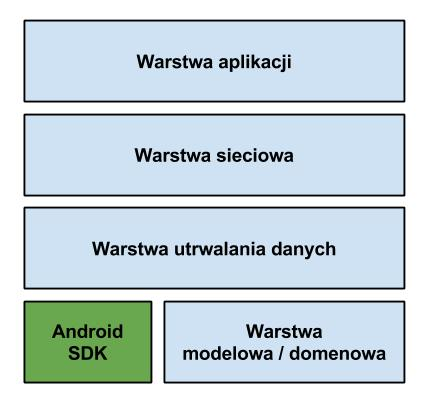
\includegraphics[width=8cm]{imgs/ch3_opis_problemu_1.jpg}
    \caption
{Podejście „standardowe” przy tworzeniu aplikacji dla systemu Android}
    \label{fig:opis_problemu}
\end{figure} 

Czyli, na najniższej warstwie położony jest Android SDK i~na niej budowane są kolejne warstwy. Każda z~kolejnych warstw oprogramowania korzysta z~warstwy poniżej, a~co za tym idzie, dziedziczy również zależności z~warstwy Android SDK. Analizując taką strukturę aplikacji dostępnych pod Androidem można zaobserwować, że w~wielu z~nich:
\begin{itemize}
\item
nie jest zachowana zasada pojedynczej odpowiedzialności,
\item
warstwa odpowiedzialna za logikę domenową jest pomieszana z~warstwą UI (User Interface),
\item
logika UI jest pomieszana z~asynchronicznym pobieraniem danych,
\item
funkcje \textit{callback\footnote{Wywołanie zwrotne (ang. callback) jest to technika programowania będąca odwrotnością wywołania funkcji. Zwykle korzystanie z~właściwości konkretnej biblioteki polega na wywołaniu funkcji (podprogramów) dostarczanych przez tę bibliotekę. w~tym przypadku jest odwrotnie: użytkownik jedynie rejestruje funkcję do późniejszego wywołania, natomiast funkcje biblioteki wywołają ją w~stosownym dla siebie czasie. \textit{"Wywołanie zwrotne", Wikipedia, 2015}}} można znaleźć w~całym kodzie,
\item
elementy warstwy UI: Activity i~Fragmenty potrafią mieć tysiące linii kodu,
\item
w większości plików aplikacji na każdej warstwie istnieją odwołania do środowiska Android,
\item
i ostatnie, ale najważniejsze z~punktu widzenia tej pracy: brak testów jednostkowych.
\end{itemize}

Spowodowane jest to dwoma czynnikami: pierwszy to trudność w~wyodrębnieniu obszarów testowych z~powodu zbyt dużego sprzężenia między warstwami (\textit{couplingu}), a~drugi – pracochłonność w~pisaniu testów. Jeżeli granica pomiędzy kolejnymi warstwami oprogramowania nie jest jasno wyznaczona, liczba testów do zaprojektowania rośnie drastycznie.

\section{Trudności w~testowaniu aktualnej struktury \newline aplikacji}
\label{testowanie_starej_struktury}

Weźmy dwie funkcjonalności: funkcjonalność \textbf{A} opisaną za pomocą kodu z~jedną instrukcją warunkową \textit{„if”}, oraz funkcjonalność \textbf{B}, w~której mamy dwie zależne od siebie instrukcje \textit{„if”}, czyli cztery możliwe decyzje programowe. Testując te funkcjonalności razem (z powodu sprzężenia nie mamy innego wyjścia) należy wykonać łącznie 
\[2*4=8\]
testów. Testy te równocześnie przestają być testami jednostkowymi, gdyż łączą w~sobie kilka funkcjonalności i~stają się przez to testami integracyjnymi. Testując natomiast te funkcjonalności osobno, trzeba wykonać 
\[2+4=6\]
testów jednostkowych. w~tym przykładzie oczywiście nie widać zbyt wielkiej optymalizacji, ale w~aplikacjach z~kodem, który dostarcza setki czy tysiące decyzji, różnica będzie znacząca.

\begin{figure}[!htb]
    \centering
    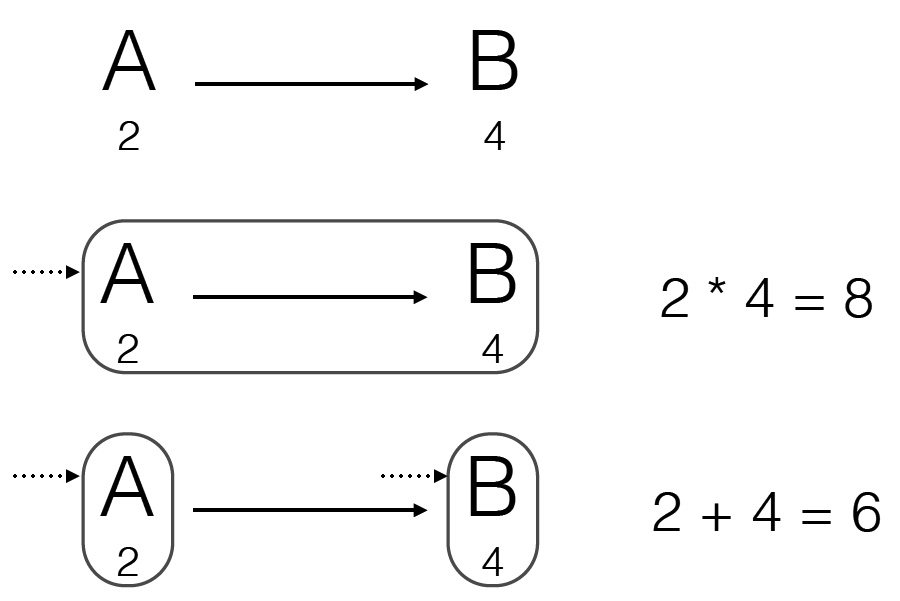
\includegraphics[width=10cm]{imgs/ch3_przyklad_testowania_klas_pl.png}
    \caption
{Różnice w~testowaniu klas osobno i~razem. \textit{"Integrated Tests are a~Scam"} - schemat autorstwa J.B. Rainsbergera \cite{website:android:testowanieklas}.}
    \label{fig:testowanie_klas}
\end{figure} 

Również w~przypadku architektury aplikacji Android, jeżeli zachodzi konieczność testowania każdej klasy lub pojedynczej funkcji w~powiązaniu z~\textit{Android SDK}, liczba testów jednostkowych zauważalnie wzrośnie.

\section{Idealna i~odwrócona piramida testowania}
\label{piramida_testowania}
Z doświadczenia własnego autora oraz innych testerów można wywnioskować, że jeżeli aplikacja ma być przetestowana zaczynając od testów integracyjnych zamiast od testów jednostkowych, nakład pracy będzie zdecydowanie większy, niż gdy zastosowany zostanie schemat standardowy, czyli zaczynając od \textit{Unit Tests}, kontynuując poprzez testy integracyjne, następnie systemowe, a~kończąc na akceptacyjnych (etapów może być więcej). 

Pozbawiając się możliwości zastosowania testów jednostkowych na wczesnym etapie projektu z~powodu źle zaprojektowanej struktury aplikacji, ryzykujemy utratę jakości, a~co za tym idzie - utratę zaufania klientów do naszego oprogramowania. Idealna piramida testowania, spopularyzowana przez Mike’a Cohna \footnote{Mike Cohn jest jednym twórców metodologii tworzenia oprogramowania Scrum. Jest jednym z~założycieli Scrum Alliance oraz właścicielem Mountain Goat Software, firmy, która oferuje szkolenia na Scrum i~technik Agile.}  w~książce „Succeeding with Agile” \cite{bib:cohn:agile}, przedstawiona została na rysunku \ref{fig:idealna_piramida}.

\begin{figure}[!htb]
    \centering
    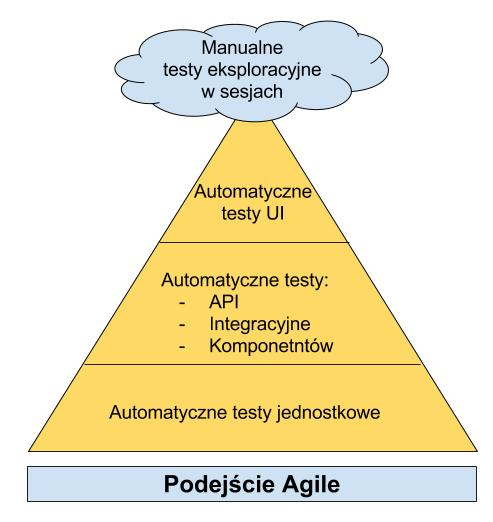
\includegraphics[width=8cm]{imgs/ch3_idealna_piramida.jpg}
    \caption
{Idealna piramida testowania według Mike'a Cohna\cite{bib:cohn:agile}.}
    \label{fig:idealna_piramida}
\end{figure} 

\newpage
Z powyższego schematu wynika, że idealnie byłoby, gdyby wszystkie etapy testów zostały zautomatyzowane (wszystkie, z~wyjątkiem manualnych testów akceptacyjnych, ale w~idealnym świecie powinno być ich tak mało, że ich automatyzacja nie miałaby większego sensu). Oczywiście piramida ta może przybierać różne formy, poziomów testowania może być więcej lub mniej, mogą być one zautomatyzowane lub nie, ale idea jest cały czas ta sama: najwięcej przypadków testowych powinno być na najniższym poziomie. Powinny być one również najprostsze do zaprojektowania. Im dalsza faza projektu, tym testy stają się bardziej pracochłonne, a~koszt usunięcia znalezionego błędu wyższy, do czego autor nawiązał już w~tabeli \ref{tab:koszty_bledu}.

Analizując aktualną strukturę większości aplikacji androidowych, schemat ten wygląda jednak tak jak na rysunku \ref{fig:odwrocona_piramida}.

\begin{figure}[!htb]
    \centering
    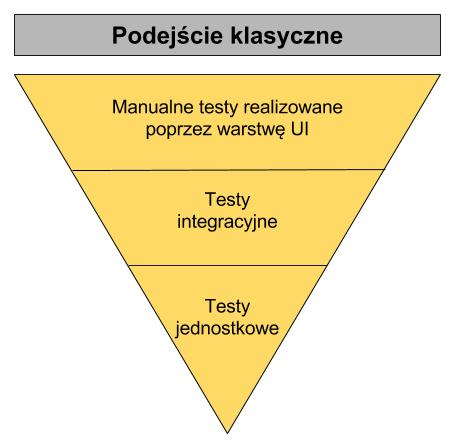
\includegraphics[width=8cm]{imgs/ch3_odwrocona_piramida.jpg}
    \caption
{Podejście klasyczne do testów, czyli odwrócona piramida testowania (\textit{Ice Cream AntiPatern}) \cite{website:piramidatestow}.}
    \label{fig:odwrocona_piramida}
\end{figure} 

\newpage
Na rysunku \ref{fig:odwrocona_piramida} widać, że z~powodu zbyt dużego \textit{couplingu} unit testy zastąpione zostają testami integracyjnymi, a~najwięcej przypadków testowych wykonywanych jest na interfejsie użytkownika (w czym znacznie pomagają frameworki testowe pozwalające na zautomatyzowanie pewnych czynności, nagranie makr według specyfikacji lub \textit{„user stories”}) oraz testy manualne.

Autor nie zaprzecza, że tym sposobem nie da się dobrze przetestować aplikacji, szczególnie jeżeli zastosujemy taktyki testowania opisane w~rozdziale \ref{testowalnosc}. Jak powszechnie wiadomo, testowanie gruntowne nie jest możliwe, jakiejkolwiek metody nie użylibyśmy. Lecz ryzyko znalezienia błędu na dalszym etapie projektu jest w~tym przypadku znacznie większe niż w~przypadku oprogramowania o~usystematyzowanej strukturze, a~co za tym idzie – koszty jego usunięcia są również znacznie wyższe.

Okazuje się, że strukturę aplikacji Android da się jednak przeprojektować tak, aby ułatwić pracę zarówno programistom jak i~testerom. Propozycja zmiany struktury aplikacji Android zaproponowana została w~rozdziale \ref{clean_architecture}

\section{Przyczyny rezygnacji z~testów jednostkowych}
\label{testy_jednostkowe_brak}
Trudna w~testowaniu struktura aplikacji to jednak nie jedyna przyczyna niedostatecznej ilości testów jednostkowych, a~nawet ich braku w~procesie tworzenia aplikacji. Przyczyn takiej sytuacji może być wiele, a~najważniejsze z~nich, zdaniem autora, to:
\begin{itemize}
\item
Niedostateczna znajomość języka programowania wśród programistów

Jeżeli programista, nawet dobry, został zmuszony przez sytuację do poznawania nowego języka programowania, to w~pierwszej kolejności chciałby, aby jego kod się kompilował, a~program zaczął działać. Jeżeli zaczyna pisać testy, to znaczy, że ma na to czas i~nie musi zagłębiać się w~techniki konfiguracji kompilatora, czy środowiska programistycznego. 

\item
Słaba znajomość narzędzi testowych

Jeżeli programista nie doskonali się w~temacie projektowania testów, nie poznaje narzędzi testowych, które mogą spowodować, że testowanie stanie się łatwe i~przyjemne, szybko zniechęci się już przy pierwszej próbie napisania trudniejszego testu, czy próbie \textit{zamockowania} jednego z~interfejsów.

\item
Niska jakość kodu źródłowego

Kiepsko zaprojektowany kod i~niezbyt optymalnie zaprojektowana architektura systemowa powoduje, że nie ma możliwości w~rozsądnym czasie przygotować zestawu testów. To powoduje, że firmy rezygnują z~ testów jednostkowych na rzecz testów integracyjnych i~systemowych, co pokazane zostało na rysunku \ref{fig:odwrocona_piramida}.

\item
Brak czasu na testy

W dzisiejszych czasach koszty projektów informatycznych są zwykle ograniczone. w~związku z~tym programiści starają się wykorzystywać cały swój czas aż do \textit{deadline'ów} na "ulepszanie" kodu, co skutkuje brakiem czasu na testy jednostkowe.

\item
Przekonanie programistów o~własnej nieomylności

Człowiek jest omylny i~popełnia błędy, do czego już autor nawiązał w~rozdziale \ref{testowalnosc}. Niektórzy programiści nie chcą jednak przyjąć tego do wiadomości i~upierają się przy stwierdzeniach, że testy do ich kawałka kodu źródłowego nie są potrzebne.
\end{itemize}

Należy zastanowić się, czy zastosowanie jednej z~taktyk zwinnych, w~tym przypadku TDD, pozwoliłoby usystematyzować pracę nad projektem i~usunąć wszystkie powyższe przyczyny.

\section{Pielęgnowalność aplikacji Android}
\label{pielegnowalnosc_aplikacji}
W realnym świecie niestety bardzo rzadko mamy możliwość tworzenia aplikacji od początku. w~większości przypadków programiści muszą borykać się z~kodem, który ktoś już kiedyś napisał, a~dotyczy to w~zasadzie wszystkich większych projektów informatycznych. Weźmy na przykład taką aplikację jak \textit{Gmail}. Wychodzą ciągle nowe wersje, ale trudno wyobrazić sobie sytuację, że któraś z~nich została po prostu napisana od nowa. w~takich przypadkach mamy do czynienia z~tzw. \textit{kodem zastanym}.

O ile kod pisany był w~sposób przejrzysty, dobrzy programiści są w~stanie dobudować nowe części aplikacji, nawet nie mając dokumentacji do starszej części. Wiele firm programistycznych stosuje podejście, że sam kod programu jest zarówno jego dokumentacją. Rozsądne nadawanie nazw zmiennym oraz umieszczanie rzeczowych komentarzy pozwala programistom zrozumieć swoich poprzedników, a~automatycznym narzędziom w~stylu \textit{JavaDoc\footnote{Javadoc – narzędzie automatycznie generujące dokumentację na podstawie zamieszczonych w~kodzie źródłowym znaczników w~komentarzach. Javadoc został stworzony specjalnie na potrzeby języka programowania Java przez firmę Sun Microsystems. \textit{"Javadoc", Wikipedia, 2015}}} wygenerować całkiem wyczerpującą dokumentację.

Gorsza sytuacja jest z~testowaniem. Jeżeli produkt nie był tworzony z~zastosowaniem TDD, praca jaką należałoby wykonać przy pisaniu unit testów do gotowego kodu może być ogromna. Ponadto istnieje ryzyko, że tester chcąc sprostać wymaganiom osób zarządzających projektem będzie tak pisał testy jednostkowe, aby pokrywały jak największą część kodu, niekoniecznie przy tym wnosząc jakoś wartość w~sprawdzenie niezawodności aplikacji.

Jedno z~możliwych rozwiązań zaproponowane zostało w~rozdziale \ref{legacy_code}